\section*{Analyse} % (fold)
\label{sec:analyse}
Das Resultat ist in Abbildung \ref{pic:sim} dargestellt. Die dunkel gestrichelte Linie ist repräsentiert die neunte Dezille bezogen auf die durch die Farbe repräsentierte Anzahl an Köchen. Die zuvor definierte Frage \textit{Wie viele Köche müssen beschäftigt werden damit mindestens 90\% aller Gäste, 10min nach ihrer Bestellung, ihre Welfencreme bekommen?} lässt sich mit \textit{es werden drei Köche benötigt} beantworten.
\paragraph{Beobachtungen}
Aus betriebswirtschaftlicher Sicht ist es evtl. besser sich nur für zwei Köche zu entscheiden, weil der zeitliche Nachteil gegenüber drei Köche nicht groß ist (ungefähr 20 sec. bei der neunten Dezille). Eine weitere interessante Beobachtung ist, dass die größte zeitliche Verbesserung bei dem Sprung von einem auf zwei Köche zu verzechen ist. Der Median sinkt von 866,9 auf 575,5 Sekunden. Betrachtet man dazu im Vergleich die Beschleunigung beim Einsatz von sechs, statt vier Köche, hat man nur eine Verbesserung von ca. zwölf Sekunden im Median.
Dieses Verhalten kann man auch in der IT, beim Einsatz von mehreren Prozessoren beobachten. Sofern die Anwendung nicht auf mehr Prozessoren ausgelegt ist, ist die Performanceverbesserung durch den Einsatz von mehr Prozessoren nur beschränkt. 


\begin{figure}[ht]
  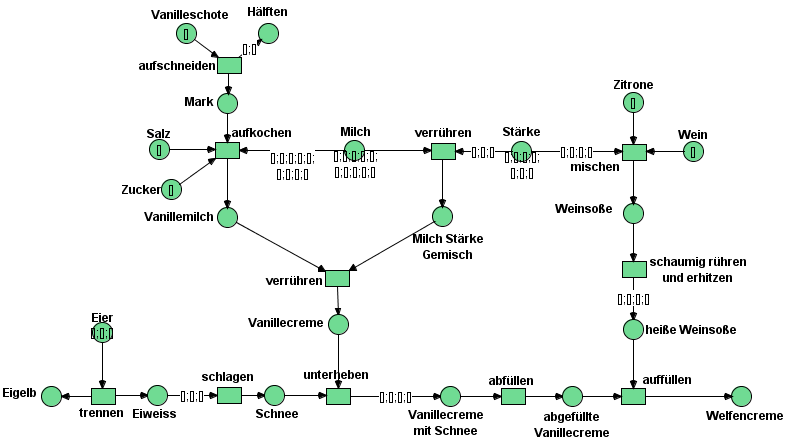
\includegraphics[width=1\textwidth]{pics/sim.png}
  \caption{Histogramm: Die Simulation des Petrinetzes mit verschiedener Anzahl Köchen, gepunktet der korrespondierende Median, dunkel gestrichelt 9. Dezille}
  \label{pic:sim}
\end{figure}


% Wie haben wir die Daten gewonnen ?
% Autohotkey ...
% java -jar loader.jar gui > data.txt

%Denk an die Fragestellung die ich aufgestellt habe und sag in wie weit die Ergebnisse auf eine reale Arbeitsumgebung anwendbar sind (nur bedingt ...)

% 9. Dezille heißt, dass 90% der Werte unterhalb dieses Wertes liegen und 10% drüber -> Fragestellung
